\subsection{Toy models}
Going back to \cref{fig:res:changing_character} we see the classical example of level crossing in two-level systems. The phenomenon gets its name because in a plot of energy versus interaction strength, the energy levels appear to cross or avoid crossing each other, depending on the specific parameters and interactions involved, as seen. Taking a look at the coefficients, we see that for small interaction strengths $\lambda$, the ground state and excited state are almost purely dominated by $\ket{0}$ and $\ket{1}$ respectively. Increasing $\lambda$, the domination is less and less present. This continues until we reach $\lambda = 2/3$, where the ground state energy is maximal and excitation energy minimal. Moving past  $\lambda = 2/3$ results in the ground state being dominated by $\ket{1}$ and the excited state by $\ket{0}$, meaning that the states has change or swapped character.


\begin{figure}
    \centering
    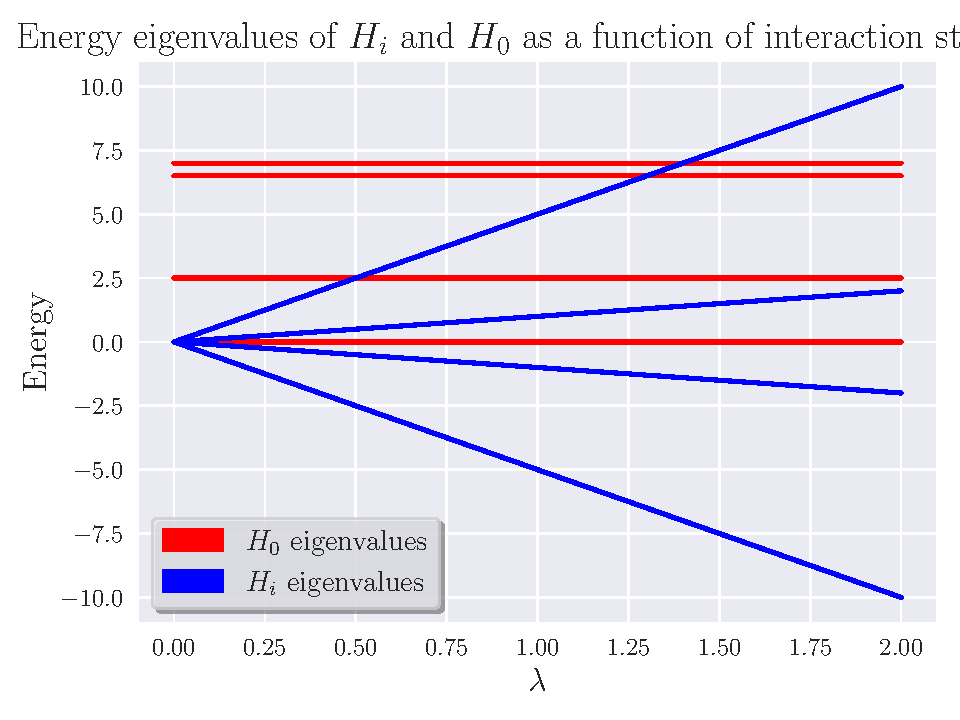
\includegraphics[scale=0.4]{figs/Eig_lmd.pdf}
    \caption{Caption}
    \label{fig:eig_lmd}
\end{figure}
The entropy in Fig. (\ref{fig:entropy}) has an initial contribution which increases slower, before taking a leap for a connection strength of $\lambda \approx 0.4$. This is probably a jump corresponding to a system being slightly interacting into being entangled. The entanglement further increases before converging around $\lambda \approx 1.3$. Studying Fig(\ref{fig:eig_lmd} Overlap) we can extract some information, seeing as the first jump is correlated with the eigenvalues of the interaction Hamiltonian overcoming the second lowest eigenvalues. The convergence can be interpreted as the interaction energy overcoming the higher eigenvalues of the non-interaction Hamiltonian.
\newline\newline

The decision of the ansatz in Fig. (\ref{fig:ansatz}) seems a bit arbitrary, but is based on the ansatz in Hlatshwayo et al. (\cite{hlatshwayoSimulatingExcitedStates2022}). There could be possibilities in optimization by choosing a different ansatz. This would be a section of further research by delving into a review of VQE by Tilly et al. (\cite{VQE_review}). \newline 
Further research could look into other methods of optimization, other than the VQE algorithm, as it is a fairly simple model with restricted applicability. It could probably be extended to solving other optimization problems with minor tweaks or clever encoding. The Lipkin model is fairly limited when it comes to QC. This is a result of the angular momentum operators $j_+$ and $j_-$ are not unitary and thus not applicable to general QC. Thus other models could be further researched in order to not simplify the Hamiltonian by non-unitarity. These models become fairly complex quickly and involves heavier computational costs in order to construct and optimize. \comment{Mangler litt idé om fler ting å kunne ta opp her.} 

\subsection{Lipkin Model}
From \cref{fig:res:Lipkin_N2_vary_v} we see good agreement between diagonalization and VQE. There were little trouble with convergence and precise results were obtained after just 30 iterations. The variability between runs were also minuscule, except when running for less than 30 iterations. It is also clear that VQE beats both HF and RPA consistently for the range of interaction strengths. 

Moving on to the four particle case from \cref{fig:res:Lipkin_N4_vary_v}, the precision of the results decreases. The two qbit scheme making use of the $W=0$ symmetry still shows excellent agreement with the diagonalization, but the larger four qbit scheme performs worse. This was the case despite increasing the number of iterations to 1000. Still, the four qbit results outperformed both HF and RPA for all except two interaction strengths, but showed some variability in results across identical runs. We hypothesize multiple reasons for this. Firstly, the number of Pauli string from \cref{eq:met:lipkin_N4_dumb} is 16 compared to the encoding from \cref{eq:met:lipkin_N4_smart_hamiltonian} only containing 6. We are therefor reliant on good estimates of Pauli string expectation values for more terms. If one or more of these estimates are poor for one iteration, the gradient estimate or the energy evaluation itself could be erroneously, resulting in slower converge. Intertwined with this is the sice of the parameter space which is twice as large for the four qbit case. Optimization here is harder and could hinder the convergence of the VQE. The $RY$ ansatz could of course also be too naive, restricting to only real amplitudes. Various different approaches are present in the literature, for instance the popular Unitary Coupled Cluster \citep{peruzzoVariationalEigenvalueSolver2014} being one of the gold standards in quantum chemistry. 
The runtime also increased with more qbits as expected. This is a clear indication that spending time reducing the number of Pauli strings by considering the symmetries of the system at hand is a worthwhile task.

Moving forward, calculations of other observable than the energy for ground state would be interesting. While the VQE is primarily focused on energy estimation, it can also yield approximate estimates for other observables, especially if they are closely related to the energy. This is because the optimized trial state tends to capture some aspects of the true state, which can influence the values of other observables. However, the accuracy of these estimates may vary depending on the specific system and observable of interest.
\begin{itemize}
    \item \st{Good correspondence for two qbit calculations. Beating both RPA and HF} 
    \item \st{Four qbits vary more. Can get differing results across runs} \begin{itemize}
        \item \st{More possible outcomes of measurements}
        \item \st{Harder to optimize due to larger parameter space. More interactions required?}
    \end{itemize}  
    \item \st{Also takes longer (due to more qbits). Emphasize using identities to shorten Pauli strings}.
    \item \st{Using the $W=0$ symmetry is good for four particles. Spending time on rewriting with symmetries in mind is a good idea.} 
    \item Comment on general usable regions for $W/V$
    \item Comment on the "holes". Hinting to more optimization required. However still classical optimizer. 
    \item Compare with HF/RPA. Here the "beating" is less clear.
\end{itemize}